\documentclass[notitlepage]{report}

\usepackage{titling}
\usepackage{blindtext}
\usepackage{amsmath}
\usepackage{amsthm}
\usepackage{amssymb}
\usepackage{float}
\usepackage{graphicx}
\usepackage{subfig}
\usepackage[utf8]{inputenc}
\usepackage[english]{babel}

\newtheorem{theorem}{Theorem}

\theoremstyle{definition}
\newtheorem{definition}{Definition}[section]

\title{%
	Collectives of local decision makers\\
	\large Construction Of A Boundary Hunter
}
\author{Daniel Braithwaite\\[1cm] {Supervisor: Marcus Frean}}

\begin{document}

\begin{titlingpage}
    \maketitle
    \begin{abstract}
    Adaptive Mixtures of Local Experts \cite{jacobs1991adaptive}, presents a system which has a number of sub networks each tasked with learning a subset of the whole training data. We wish to extend this idea by making each expert network responsible for deciding what it is interested in, we call such expert networks boundary hunters. Our initial approach to a design boundary hunter was to create a loss function which promoted the learning of local features, solving this problem equates to a careful balancing of the rewards and penalties, after multiple attempts in which the boundary hunter either learnt to care about every data point or none of them we concluded that a different approach was needed. Consequently we shifted our attention to networks of boundary hunters based of Radial Basis Function (RBF) Networks, where the hidden layer of the network consisted of boundary hunters instead of RBF Neurons, this approach worked on our toy problems. Following this success we discovered that using this network structure actually reintroduced dependency between the hidden neurons, what we where trying to avoid, so we attempted to train a single boundary hunter neuron by its self which after some modifications we found to work as we had hoped for. Testing both our individual and networks of boundary hunters on the Sonar benchmark problem showed that while the ideas developed in this report are effective on small contrived examples we have yet to develop something which is able to compete with today's cutting edge neural networks.
    \end{abstract}
\end{titlingpage}

\chapter{Introduction}

Single or Multilayer Perceptron Networks are commonly trained to model and solve supervised learning problems. If however an attempt is made to train these networks to perform different tasks on different occasions then using a training algorythm such as Backpropergation will result is slow convergence and poor generalization. \textbf{Find Citation, Many papers say this but dont provide reference}

In the paper Adaptive Mixtures of Local Experts \cite{jacobs1991adaptive} an idea was proposed to create systems where one has a number of expert networks, each responsible for only a subset of the data. While training our system we want to be able to learn which expert is responsible for which data points, this is where a gating network comes in, it is trained along side our expert networks and decides who is responsible for each data point. The idea being that if our problem consists of a training set which can be naturally divided up into distinct sub problems, then using these networks will provide better performance, by approximating all of these functions separately and interpolating between them, rather than assuming the data is governed by one function and trying to learning something that does not naturally exist.\\

During training if an expert has a low responsibility for some data it is allowed to slack off and get it wrong, this means that another expert has a high responsibility for that data and must be doing its best to classify it correctly. So the expert networks are not completely independent as each one relies on the others to pick up the slack for what it gets wrong.\\

The goal of this project is to further reduce the dependence between these expert networks, we want each to be responsible for deciding what it cares about thus making it possible for us to train them individually, we will call such expert networks boundary hunters. Consider the following situation, a very contrived toy example of our motivation for this project. We have a binary classification problem with the data split by a chevron. 

\begin{figure}[H]
	\centering
	\begin{minipage}[b]{0.8\textwidth}
		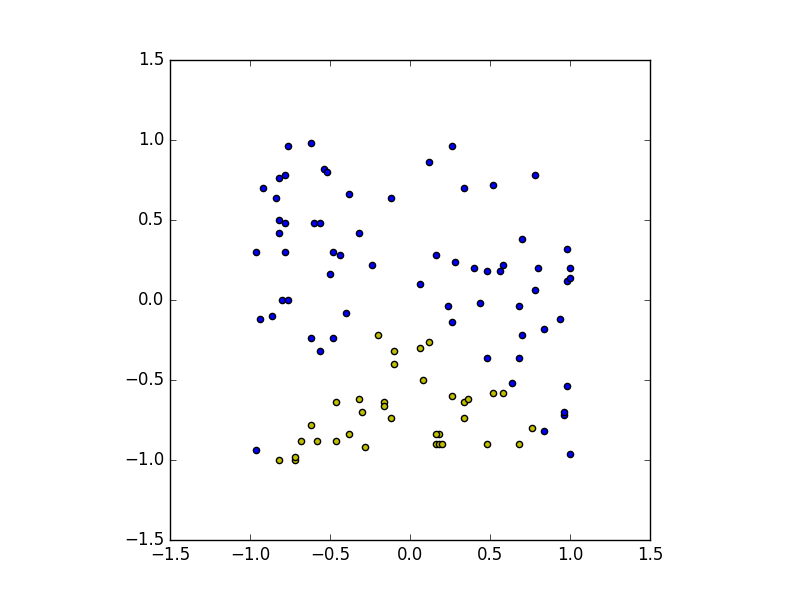
\includegraphics[width=\textwidth]{CHEV-DATA-EX.png}
		\caption{Example data for situation}
	\end{minipage}
	\hfill
\end{figure}

A single perceptron will go and place a horizontal line through the plane however this is not telling us anything interesting. And if we think about our adaptive mixtures of experts model, a system with only a single expert will simply have the one being responsible for every data point. In this situation we would like to train a boundary hunter by its self, which will identify a local feature (i.e. one side of the chevron), learn to classify it and ignore the data it cant deal with.

\chapter{Neuron Parametrisation}
A perceptron is learning a hyperplane described by its normal vector plus a bias. To define our boundary hunter we want to specify a region of interest, a logical way to do this is to specify some region around a point. This is where we arrive at a problem, namely our current parametrisation of a neuron does not have the information to do.

\section{Normal \& Point Parametrisation}
To define our radius of interest we will start by describing it as a radius around a point. Leading us to the following definition.

\theoremstyle{definition}
\begin{definition}
	The \textbf{Normal \& Point} parametrisation of a perceptron consists of the vector $n = [n_1, ..., n_k]$ normal to our hyperplane and $p = [p_1, ..., p_k]$ the point our hyperplane passes though.\\
	
	On input $x = [x_1, ..., x_k]$ to the neuron we define the weighted sum as 
	
	\begin{align*}
	z = \sum_{i=1}^k n_i \cdot (p_i - x_i)
	\end{align*}
\end{definition}

\begin{theorem}
The normal \& point representation for a perceptron is equivalent to our standard definition
\end{theorem}

\begin{proof}
Say we have some normal and point representation for a perceptron, $n = [n_1, ..., n_k], p = [p_1, ..., p_k]$, then we have $z$ as defined above

\begin{align*}
z &= \sum_{i=1}^k n_i \cdot (p_i - x_i)\\
&= n \cdot [p_1 - x_1, ..., p_k - x_k]\\
&= n_1 \cdot (p_1 - x_1) + ... + n_k \cdot (p_k - x_k)\\
&= n_1p_1 - n_1x_1 .... n_kp_k - n_kx_k\\
&= (n_1p_1 + ... + n_kp_k) - n_1x_1 - ... - n_kx_k
\end{align*}

Now we can define an equivalent standard perceptron, where we have a bias term $b = n_1p_1 + ... + n_kp_k$ and each component of the normal vector $n^{'}_i = -n_i$

\end{proof}

\subsubsection{Comparison To Perceptron}
We can compare the two experimentally to confirm our findings, using the same data and over 50,000 iterations. In the graph for our modified perceptron the green point is our vector on the hyperplane.


\begin{figure}[H]
\centering
  \begin{minipage}[b]{0.4\textwidth}
    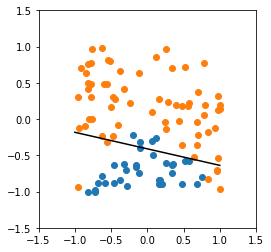
\includegraphics[width=\textwidth]{Standard-Perceptron.png}
    \caption{Standard Perceptron (SSE = 3.90)}
  \end{minipage}
  \hfill
  \begin{minipage}[b]{0.4\textwidth}
    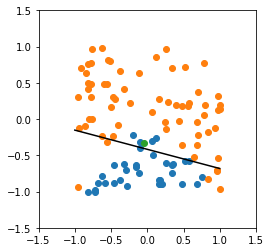
\includegraphics[width=\textwidth]{Modified-Perceptron-(Normal-Point).png}
    \caption{Modified Perceptron (SSE = 3.90)}
  \end{minipage}
\end{figure}

The figures above provide experimental evidence that our normal and point perceptron will converge to the same optimal solution as the standard one.

\chapter{Boundary Hunter: First Attempt}
Using the \textbf{Normal \& Point Parametrization} we wish to train our neurons to be boundary hunters. We propose that this can be done by constructing a loss which encourages neurons to find local features. In this chapter we explore various ideas for loss functions, learning from our mistakes along the way.

\section{Responsibility Function}
Before we construct our loss functions we need a notion for how responsible our boundary hunter is for a given data point, we denote $r_i$ the responsibility for data point $i$. We would like the following property's of a responsibility function

\begin{enumerate}
	\item We want our responsibility to lie in the interval $[0, 1]$
	\item continuous and differentiable
	\item All points inside the area of interest should have the same responsibility.
	\item Responsibility for points outside the area of interest should decrease as distance from area increases.
\end{enumerate}

Property (1) is simply because it keeps things constrained, a responsibility of 0 means we do not care at all and 1 means we absolutely care. (2) is so our gradients work nicely with Backpropagation. (3) is because if we have two points in our radius of interest then it makes sense to be equally interested in them, it defeats the purpose of having a radius if being inside it does not definitively mean that we are interested. (4) guarantees that as we move further away from the edge of our radius we get less interested.

The following function seems like a good place to start. The responsibility for any point inside the area of interest is 1, and as the data points get further away the responsibility decreases, we also satisfy property (1)

\begin{align}
r_i = 1 - \frac{max(0, d-r)}{abs(d-r) + 0.1}
\end{align}

However we note that this functions is not smooth which is certainly a result of property (3). While its reasonable for us to want property (3) any function which satisfies this will not be continuous and differentiable everywhere, hence not satisfying property (2) and causes problems when training with Backpropagation as it is computing the gradient of our loss function, because of this we will not strictly consider property (3). Now we turn to the logistic function, $f = 1 - \frac{1}{1 + e^{-S(x - x_0)}}$, where S is the steepness of our sigmoid. A nice property is that by adjusting the steepness we can get close to satisfying property (3) with a continuous function. To achieve our approximation of property (3) we want our responsibility function to have a low sensitivity at each extreme, a small change in distance when the point is either very close to or far from our centre point should have a negligible impact on the responsibility, however we want our function to be very sensitive around the border of our expertise area. By a purely arbitrary decision we will start with a steepness of 10, giving us the following formula for responsibility.

\begin{align}
r_i = 1 - \frac{1}{1 + e^{-10(x-r)}}
\end{align}

where $r$ is the radius of our area.


\section{Loss Function Design: Attempt 1}
Consider our boundary hunter as reducing the uncertainty of what we think the class is for each data point. As the data points get further away from our radius of expertises we become more uncertain about its class. So a reasonable loss function is 

\begin{align}
\frac{1}{n} \sum_{i=0}^n r_i(C_i log(y_i) + (1-C_i)log(1-y_i)) + (1-r_i) log(1/2)
\end{align}

As $r_i \rightarrow 0$ the loss for data point $i$ is weighted more toward a coin toss as the boundary hunter is becoming more uncertain about how correct it is. The opposite is true as $r_i \rightarrow 1$, now the loss becomes weighted more towards the cross entropy and thus the actual output of the boundary hunter.

\subsection{Experimental Results}
Using these loss and responsibility functions our boundary hunter learns to care about all the data. Which is certainly doing the opposite of learning local features.

\begin{figure}[H]
\centering
  \begin{minipage}[b]{0.4\textwidth}
    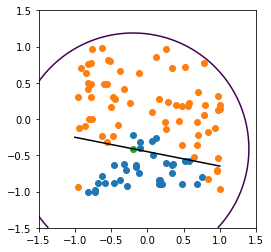
\includegraphics[width=\textwidth]{BoundaryHunter-Attempt1-01.png}
    \caption{Boundary Hunter with (3.3) as loss and (3.2) as responsibility}
  \end{minipage}
  \hfill
\end{figure}

\subsection{Justification For Results}
Consider our loss for a given data point with target $t$, prediction $y$ and responsibility $r$. Without loss of generality, assume $t = 1$. So then we are left with $r\ log(y) + (1-r)\ log(\frac{1}{2})$. We know that if we are getting it right $log(y) \leq log(\frac{1}{2})$. In this situation we are getting only a few wrong which allows the boundary hunter to take the hit for these while getting everything else right.

\subsection{Reflection}
Thinking of the problem in this way is intuitive but not strict enough in this form, we need a harsher penalty for getting things wrong to encourage the boundary hunter to have a near perfect accuracy and exclude data which compromises this.

\section{Loss Function Design: Attempt 2}
Based on our previous findings a more in depth consideration of a suitable loss function is required. Essentially we want to reward our boundary hunter if it is an expert in a given region, so if it gets things wrong outside its area of interest that's good, and if it gets things correct outside its area of interest then that's bad. Consider the following properties of our ideal loss function.

\begin{enumerate}
\item As a data point gets further away from our area of interest we "care less" about our accuracy for classifying that point.
\item Increasing area of interest should decrease the loss if and only if increasing the area of interest allows us to classify more points correctly.
\item Decreasing area of interest should decrease the loss if and only if reducing area of interest allows us to classify less points incorrectly in our area
\end{enumerate}

We can expand on these ideas to get the following

\begin{enumerate}
\item We want to be as accurate as possible in our area of interest and care less about our accuracy based on how "responsible" we are for the data point.
\item We should be penalized for classifying things correctly outside our area of interest based on how "not responsible" we are for the data point (i.e. if we are classifying a data point correctly but it is just outside our area of interest then we should be penalised).
\item We should be rewarded for classifying things incorrectly outside our area of interest based on how "not responsible" we are for the data point (i.e. if we are classifying a data point incorrectly and its just outside our area of interest then we should be rewarded).
\end{enumerate}

We now wish to convert this into a loss function. Item (1) is referring to $r_n$ multiplied by the standard cross entropy, restricted to points inside our area of interest. Items (2) + (3) are referring to the opposite of our cross entropy multiplied by $r_n$ restricted to all points outside our area of interest.

\begin{align}
- \big( \frac{1}{|I|} \big[ \sum_{i \in I} H(t_i, y_i) \big] + \frac{1}{|O|} \big[ \sum_{i \in O} H(1 - t_i, y_i) \big] \big)
\end{align}

Where $I$ and $O$ are the sets of points inside and outside our area of interest retrospectively.

\subsection{Experimental Results}

With the same set-up as before this performs horribly, not doing anything of interest.

\begin{figure}[H]
\centering
  \begin{minipage}[b]{0.4\textwidth}
    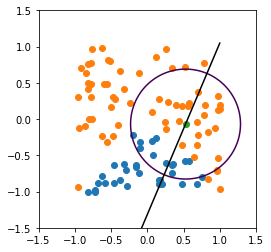
\includegraphics[width=\textwidth]{BoundaryHunter-Attempt2-01.png}
    \caption{Boundary Hunter with (3.4) as loss and (3.2) as responsibility}
  \end{minipage}
  \hfill
\end{figure}

\subsection{Reflection}
The conditions used to construct this loss are to harsh, currently we are trying to maximize our error outside the region while minimizing our error inside, really we don't care about the error outside our region, we only want to know if increasing our area will allow us to achieve a better error, supporting the use of our steep responsibility function as the points which will indicate whether we should increase our radius are the ones just on the border.

\section{Loss Function Design: Important Observation}
We take a step back and consider the basics of what we are trying to achieve. First we make an interesting observation which will change the way we approach designing this loss. Consider the simple loss function $L =\sum R(r, i) * CE(i)$ where $R(r, i)$ is our responsibility function with paramater $r$ as the radius and $i$ as the data point, $CE(i)$ is our cross entropy of data point i. Given we want the quantity $\frac{\partial L}{\partial r}$ so we can train r, we compute the following.

\begin{align*}
\frac{\partial L}{\partial r} &= \frac{\partial}{\partial r} \big[ \sum R(r, i) * CE(i) \big] \\
&= \sum R^{'} (r) * CE(i)
\end{align*} 

We observe that the quantity $\frac{\partial L}{\partial r}$ does not actually tell us how changing the radius changes our error, consider that $CE(i)$ is always positive, so essentially $\frac{\partial L}{\partial r} = \alpha * R^{'}(r)$, so it simply tells us which direction to move the radius to increase the responsibility. This results in the our area of interest constantly increasing. So we conclude that simply scaling the loss by a boundary hunters responsibility for a data point will not work.\\

\section{Loss Function Design: Attempt 3}
Based on what we just observed a new approach is needed. We consider our boundary hunter as a salesperson, who gets paid $\$B$ for selling something to someone who wants it (if the salesperson is responsible for this individual) and gets penalized $\$C$ dollars for selling something to someone who does not want it. Using this model, the salesperson is to position them selves and adjust their responsibility so that they are maximizing there profit. Now we simply must quantify this, we know $y^t(1-y)^{t-1}$ is the probability we get something right (i.e. probability we are selling to someone who wants it). We arrive at the flowing quantity.

\begin{align}
L = \sum_{i=0} r_i * \big[Cy_i^{1-t_i}(1-y_i)^{t_i} - By_i^{t_i}(1-y_i)^{1-t_i} \big] 
\end{align}

While initially it seemed like this would suffer from the same problem described in the previous observation it does not. Consider the differential $R^{'}(r)$, we know that $R^{'}(r)$ will always have the same sign but $Cy_i^{1-t_i}(1-y_i)^{t_i} - By_i^{t_i}(1-y_i)^{1-t_i}$ can be both positive and negative, so we end up in the situation where if we are losing more money than we are gaining then we will decrease our radius so we can cut our losses, otherwise if we are making a profit then we will want to increase our sales area. 

\subsection{Experimental Results}
With the same parameters as before we train a perception with this loss and find that its best solution is selling to everyone, essentially what a standard perceptron would provide.

\begin{figure}[H]
\centering
  \begin{minipage}[b]{0.4\textwidth}
    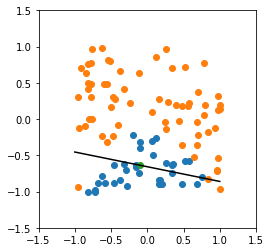
\includegraphics[width=\textwidth]{BoundaryHunter-Attempt3-01.png}
    \caption{Boundary Hunter with (3.5) as loss and (3.2) as responsibility}
  \end{minipage}
  \hfill
\end{figure}

Not quite the results we where looking for but this outcome makes sense, the solution presented gets many more points correct than it does wrong, so the boundary hunter is fulfilling its goal of making a maximal profit. Increasing the parameter C will allow us to tune our boundary hunter to care more about getting things incorrect. To get a good spread we use C = 2, 2.5, 3

\begin{figure}[H]
  \centering
  \begin{minipage}[b]{0.49\textwidth}
    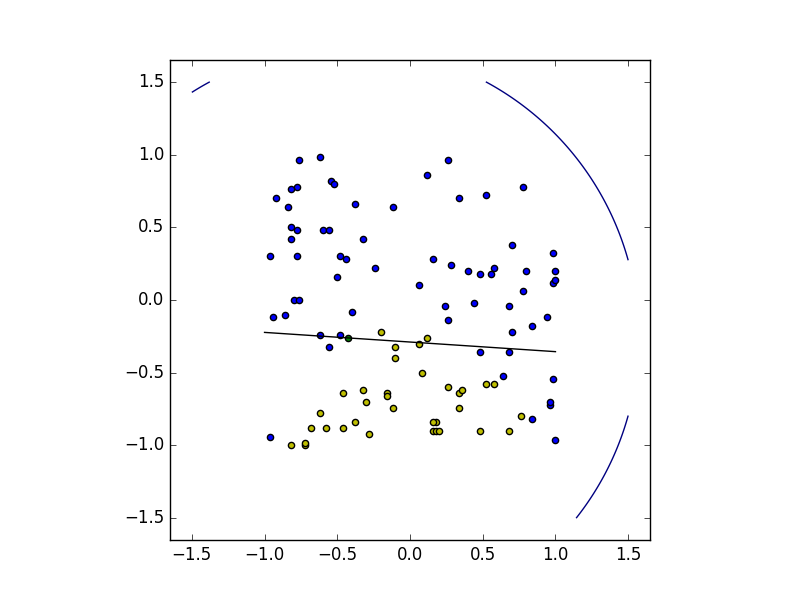
\includegraphics[width=\textwidth]{BoundaryHunter-Attempt3-02.png}
    \caption{C = 1.3}
  \end{minipage}
  \hfill
  \begin{minipage}[b]{0.49\textwidth}
    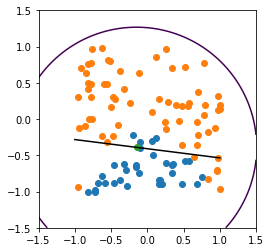
\includegraphics[width=\textwidth]{BoundaryHunter-Attempt3-03.png}
    \caption{C = 1.6}
  \end{minipage}
  \hfill
  \begin{minipage}[b]{0.49\textwidth}
    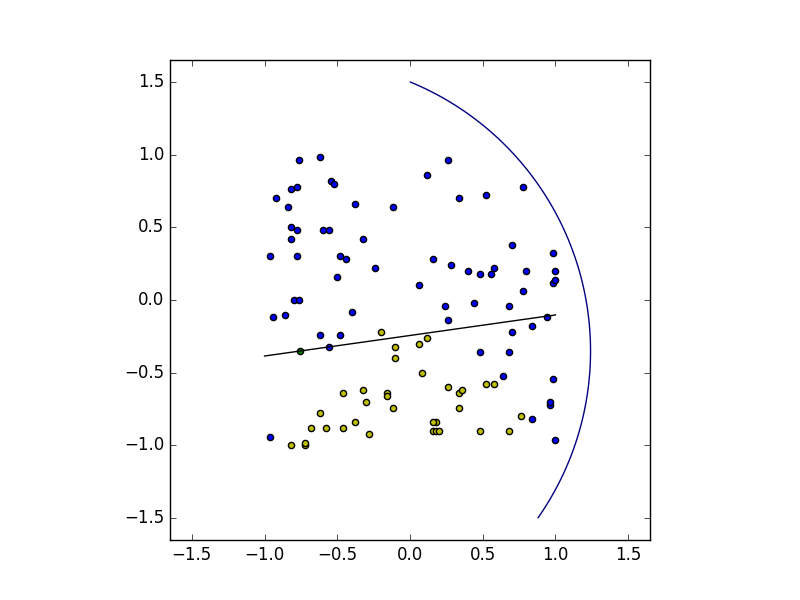
\includegraphics[width=\textwidth]{BoundaryHunter-Attempt3-04.png}
    \caption{C = 1.9}
  \end{minipage}
\end{figure}

However this only seems to change the hyperplane positioning and not solve the issue of our radius including everything. If we impose some reasonable restrictions on the radius (i.e. $0.3 \leq r \leq 0.8$), set our C = 2 and adjust the responsibility function to be less steep (steepness of 5) then we can achieve some better results which are more in line with our goal.

\begin{figure}[H]
  \centering
  \begin{minipage}[b]{0.4\textwidth}
    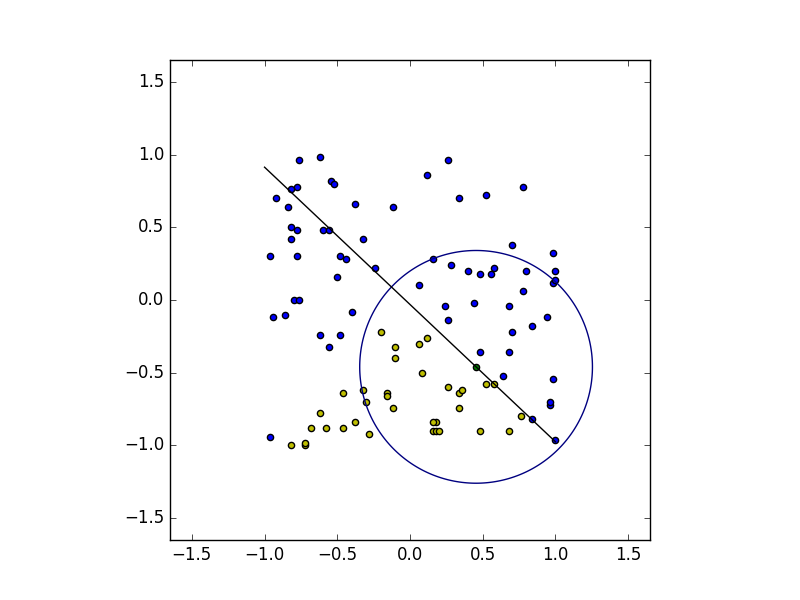
\includegraphics[width=\textwidth]{BoundaryHunter-Attempt3-R0.png}
    \caption{}
  \end{minipage}
  \hfill
  \begin{minipage}[b]{0.4\textwidth}
    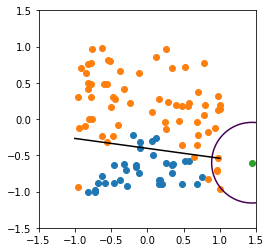
\includegraphics[width=\textwidth]{BoundaryHunter-Attempt3-R1.png}
    \caption{}
  \end{minipage}
  \hfill
\end{figure}

However more often than not we get results like following, which do not achieve anything useful or meaningful.

\begin{figure}[H]
  \centering
  \begin{minipage}[b]{0.5\textwidth}
    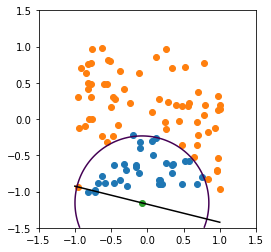
\includegraphics[width=\textwidth]{BoundaryHunter-Attempt3-R2.png}
    \caption{}
  \end{minipage}
  \hfill
\end{figure}

The issue appears to be that of local optima, the solutions looking like what we want (Figure 3.7 and 3.8) certainly have lower error than when the solution is outside the data however our boundary hunter appears to have trouble escaping local optima to find these more interesting solutions.

To confirm this we look to plot the landscape of our loss function, we will fix the radius and hyperplane position while varying the x and y coordinates of the point. These fixed parameters represent the hyperplane and radius we would want if trying to place our self on the left side of the chevron. Using a steepness of 5 and C = 2 we get the following plots.

\begin{figure}[H]
  \centering
  \begin{minipage}[b]{0.8\textwidth}
    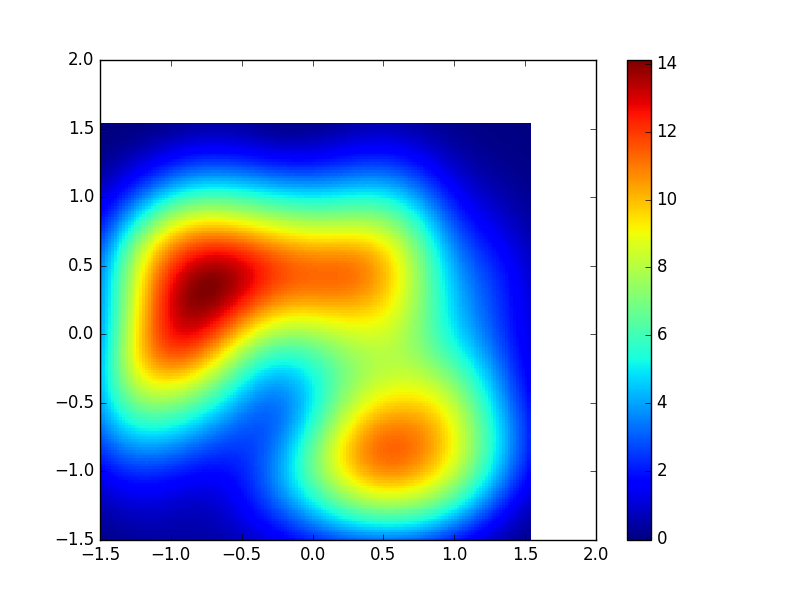
\includegraphics[width=\textwidth]{LossPlot-1.png}
    \caption{Radius as 0.3}
  \end{minipage}
  \hfill
\end{figure}

\begin{figure}[H]
  \centering
  \begin{minipage}[b]{0.8\textwidth}
    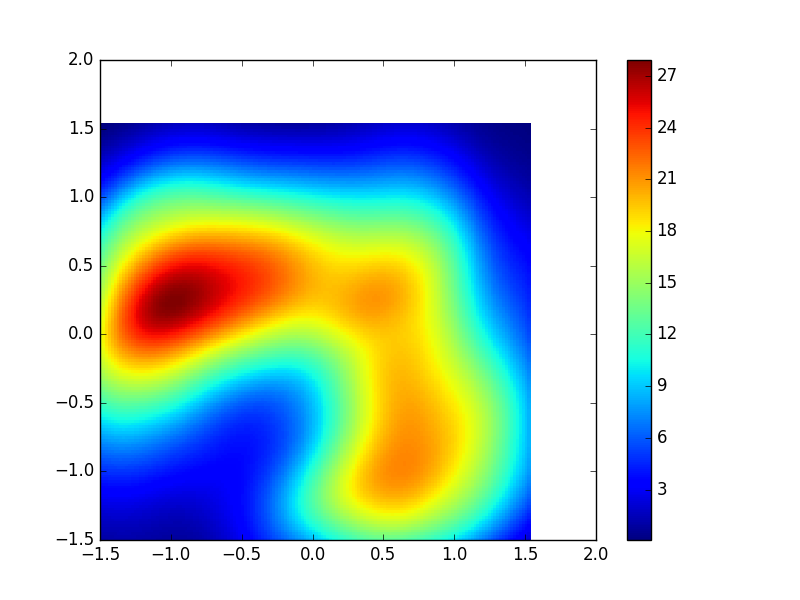
\includegraphics[width=\textwidth]{LossPlot-2.png}
    \caption{Radius as 0.8}
  \end{minipage}
  \hfill
\end{figure}

\begin{figure}[H]
  \centering
  \begin{minipage}[b]{0.8\textwidth}
    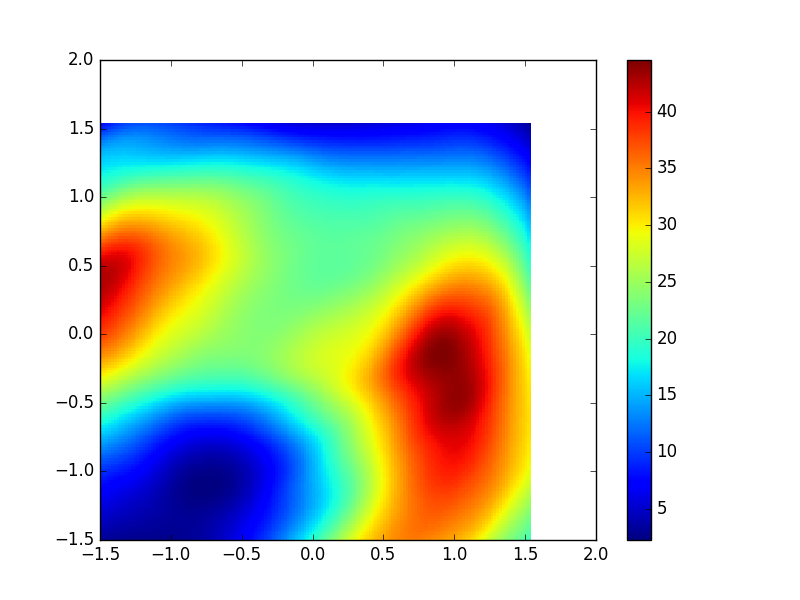
\includegraphics[width=\textwidth]{LossPlot-3.png}
    \caption{Radius as 2.0}
  \end{minipage}
  \hfill
\end{figure}

As clearly demonstrated by these graphs this loss function is not conducive to finding the optimal solution we are expecting.  There is a noticeable deformation in the contour where our expected solution is, however it is unlikely that it will be found by the boundary hunter, more often than not we will end up outside of the data. For points outside our area of interest the responsibility rapidly approaches 0, this is what would cause the edge to be an optimal solution. While this would indicate a responsibility function which is to steep.

\begin{figure}[H]
  \centering
  \begin{minipage}[b]{0.8\textwidth}
    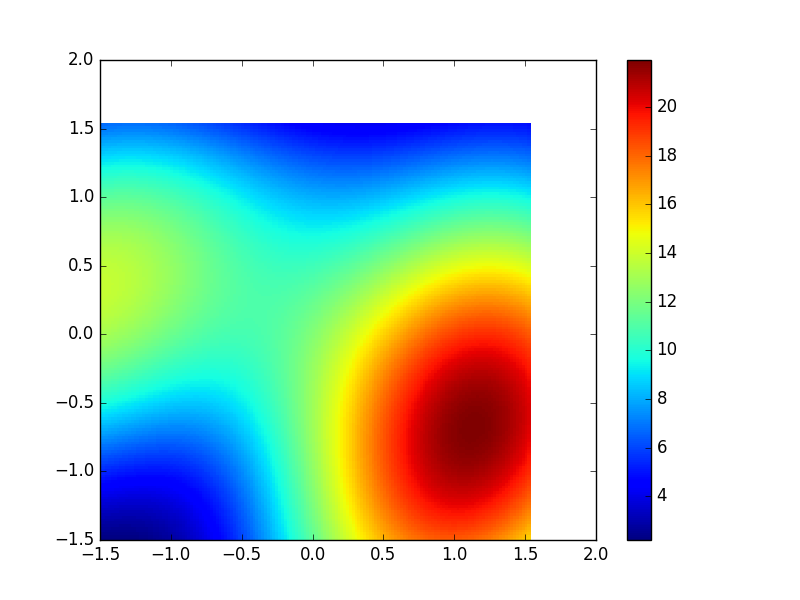
\includegraphics[width=\textwidth]{LossPlot-4.png}
    \caption{Radius as 0.3, with steepness as 0.5}
  \end{minipage}
  \hfill
\end{figure}

Even with a significantly less steep responsibility function we still have the same landscape. 

\section{Discussion}
These results from this section leads me to believe a new approach is needed, simply trying to incorporate the responsibility into a loss function is, in essence a careful balancing act of rewards and penalty's for which there is possibly no solution. We need to investigate something other than simply designing a new loss function.

\chapter{Radial Basis Function Networks}
We turn our attention to a class of networks which seem very closely related to what we want, these are Radial Basis Function (RBF) Networks. Before we can talk about RBF Networks we will first define what an RBF is.\\

The output of a \textbf{Radial Basis Function} depends only on the distance from its input to some point we call the centre of the RBF. $f(x, c) = f(\lVert x - c \lVert)$.\\

And then we can define the activation of a RBF Neuron as being a function satisfying the properties of an RBF. Essentially each RBF Neuron is measuring the similarity between its centre and the input vector presented to it, the closer the input is to the centre the closer the activation is to 1. Any RBF will do as an activation but we will be using one based on a the 1D Gaussian distribution. The equation for a 1D Gaussian is 

\begin{align*}
f(x) = \frac{1}{\sigma \sqrt{2 \pi}} e^{-\frac{(x-\mu)^2}{2\sigma^2}}
\end{align*}

We can make some simplifications seeing as we aren't interested in the standard deviation, making our activation

\begin{align}
a(x) = e^{-\beta \lVert x - c \lVert}
\end{align}

We use the $\beta$ term to control how quickly the activation decays.\\

An intuitive view of an RBF network is we have a number of RBF Neurons in the hidden layer which tells the output layer how close the input vector is to its centre, the output neurons then use this information to make a decision about their activation by taking a weighted sum of the outputs from the hidden layer.

\section{Training RBF Networks}
We will use the simplest method for training an RBF Network. Simply randomly initialize all the parameters of our network and then use gradient descent to find better ones. Using this method we are able to achieve good classifiers for data. 

\begin{figure}[H]
  \centering
  \begin{minipage}[b]{0.4\textwidth}
    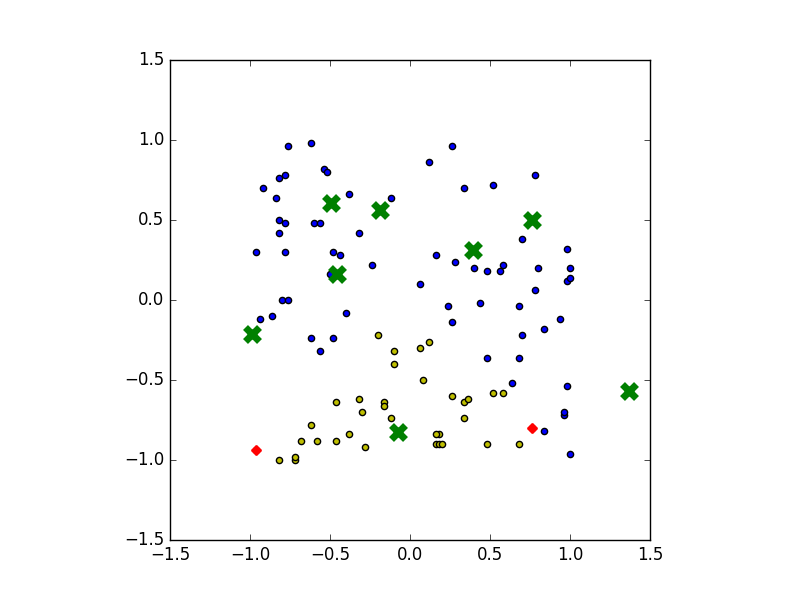
\includegraphics[width=\textwidth]{RBFN-01.png}
    \caption{}
  \end{minipage}
  \hfill
  \centering
  \begin{minipage}[b]{0.4\textwidth}
    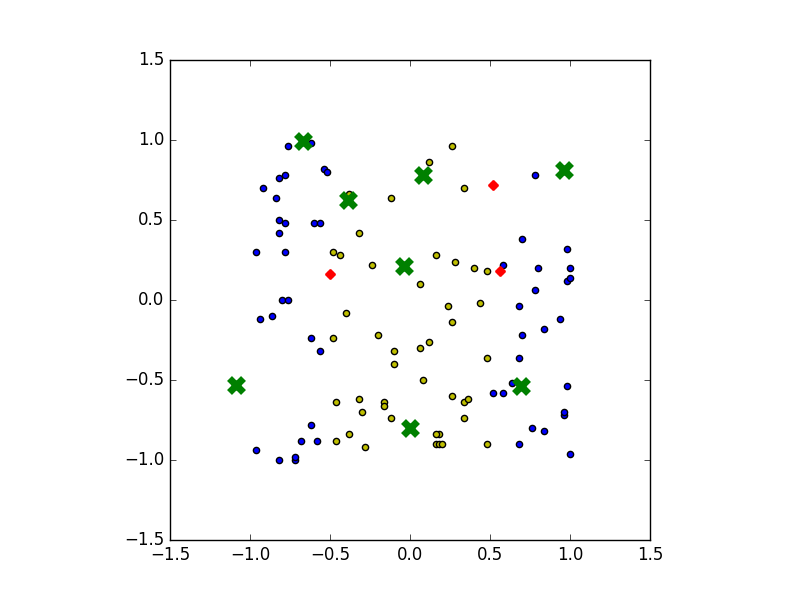
\includegraphics[width=\textwidth]{RBFN-02.png}
    \caption{}
  \end{minipage}
  \hfill
  \centering
  \begin{minipage}[b]{0.4\textwidth}
    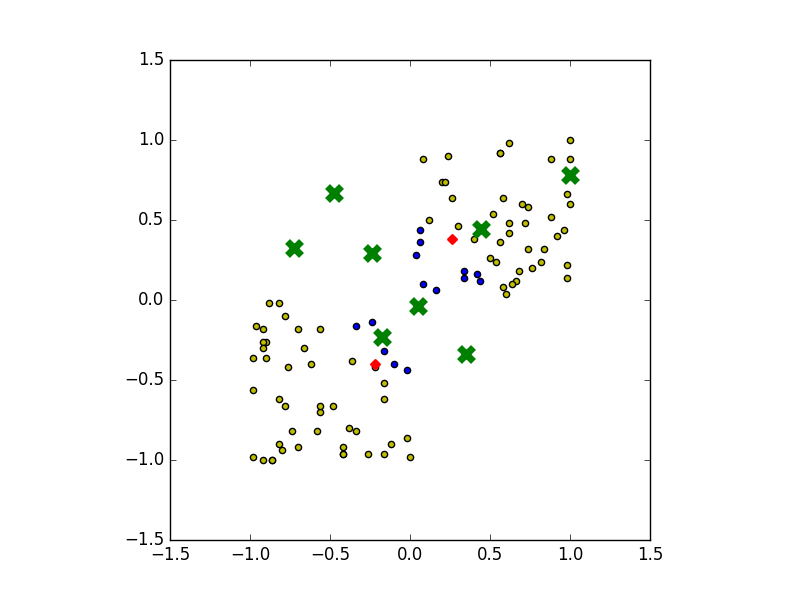
\includegraphics[width=\textwidth]{RBFN-03.png}
    \caption{}
  \end{minipage}
  \hfill

The green x's and red x's represent our centroids and the points we are getting incorrect retrospectively
\end{figure}

One can see that some of the RBF Neurons are placed in the centre of interesting points in the data.

\section{Discussion}
How can we convert the idea of these RBF Networks into boundary hunters? At the moment we have networks in which the hidden neurons don't classify point, they simply report to the output layer how confident they are that the input is in there radius. The RBF Neurons are trying to locate interesting blobs of data and position themselves in the middle.

\chapter{RBF Based Boundary Hunters}
Based on these RBF Networks, is it possible to use the ideas that we had previously to construct a boundary hunter? In this chapter we create the concept of a RBF Boundary Hunter Neuron and derive an activation function.\\

Consider that the output of a regular RBF Neuron is the uncertainty about whether the given point is within its radius, as the point gets further away we become less certain about our ownership and so the activation decreases in value. We would like to incorporate this into the output of our RBF Boundary Hunter as the points move further away from the centre then we become less sure about our classification. Let $f$ be our activation function, as our belief that the point is in class 1 increases $f \rightarrow 1$ and as it decreases we have $f \rightarrow 0$, so if $f = \frac{1}{2}$ then we are unsure about the class of a point. It seems logical for $f \rightarrow \frac{1}{2}$ as the distance between our centre of a boundary hunter and a point increases. Now we can define our RFB Boundary Hunter Neuron for binary classification.\\

\theoremstyle{definition}
\begin{definition}
A \textbf{RBF Boundary Hunter Neuron} (for binary classification) in $\mathbb{R}^n$ has $2n + 1$ free parameters. $\beta \in \mathbb{R}$, $\mathbf{c} \in \mathbb{R}^n$ and $\mathbf{n} \in \mathbb{R}^n$. $\beta, \mathbf{c}$ represent decay speed and centre of the RBF portion of our neuron. $\mathbf{n}$ defines a hyperplane which passes through our point $\mathbf{c}$. We define the activation as follows

\begin{align}
a(x) &= \frac{1}{2} + e^{-\beta \lVert x - c \lVert^2}(\frac{1}{1 + e^{-(\mathbf{n} \cdot (\mathbf{c} - x))}} - \frac{1}{2})
\end{align}

\end{definition}

\subsection{Training RBF Boundary Hunters}
Using the same method as before, randomly initializing all parameters and then training using gradient descent. Although we must clip our betas to be positive, undesirable but necessary, if we don't clip them then the value outputted by the gate explodes.

\begin{figure}[H]
  \centering
  \begin{minipage}[b]{0.4\textwidth}
    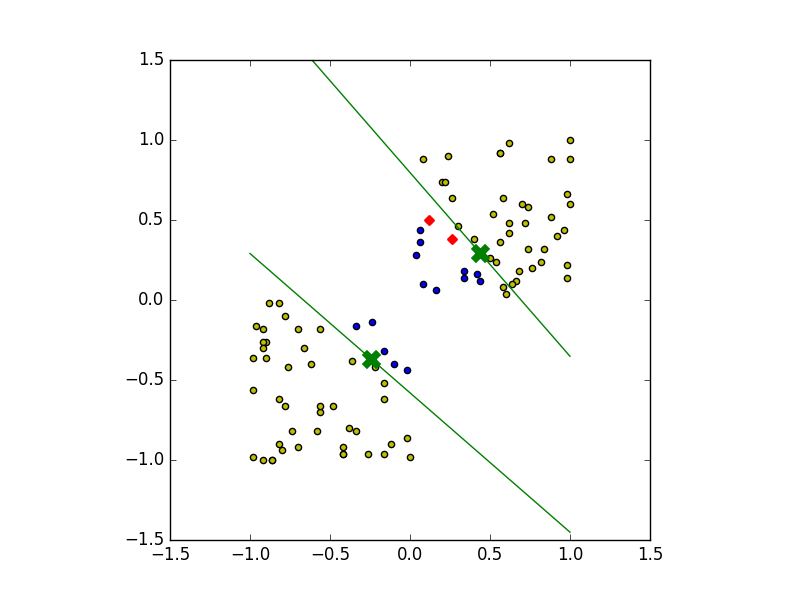
\includegraphics[width=\textwidth]{RBFN-BH-01.png}
    \caption{}
  \end{minipage}
  \hfill
  \centering
  \begin{minipage}[b]{0.4\textwidth}
    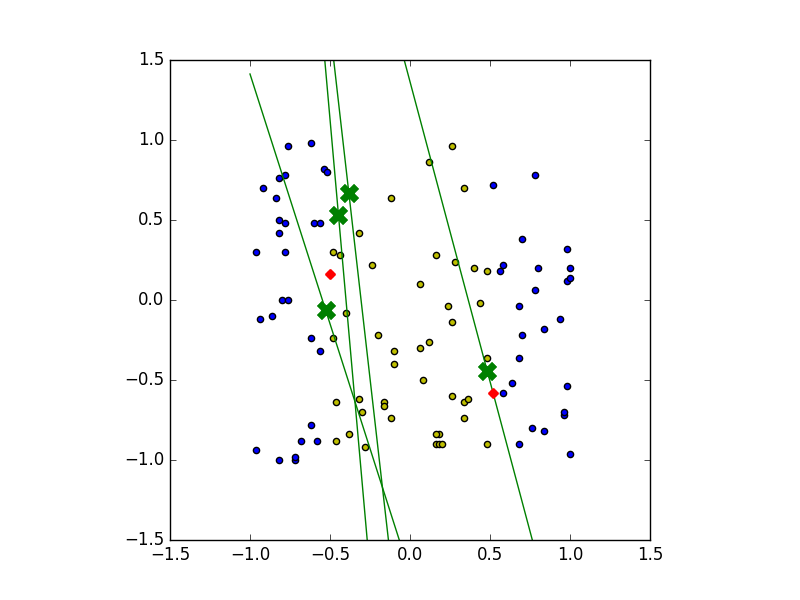
\includegraphics[width=\textwidth]{RBFN-BH-02.png}
    \caption{}
  \end{minipage}
  \hfill
  \centering
  \begin{minipage}[b]{0.4\textwidth}
    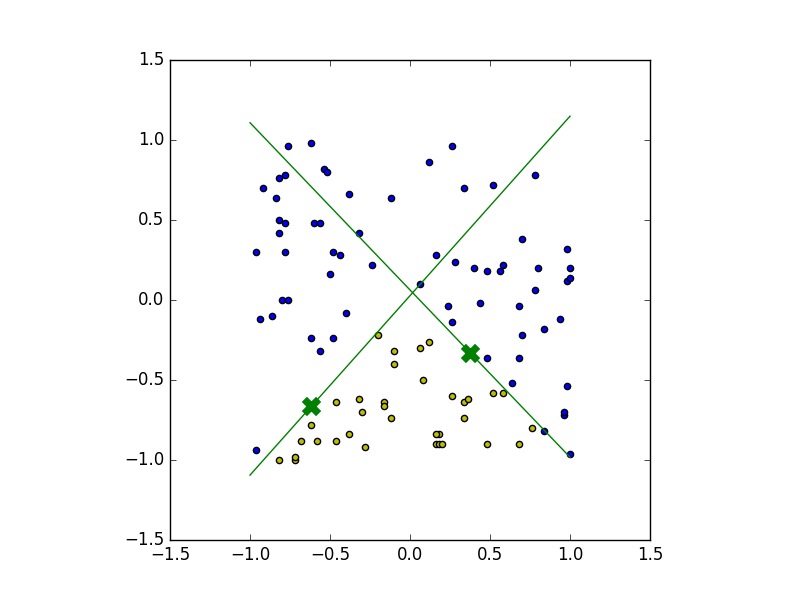
\includegraphics[width=\textwidth]{RBFN-BH-03.png}
    \caption{}
  \end{minipage}
  \hfill

The green x's represent our centroids while the red x's represent the points we are getting incorrect
\end{figure}

These are promising and consistent results. The hyperplanes being placed exactly where we would hope, however because the final decision is made by the output layer some results are a little mysterious to understand. Returning to our motivation for this project, what happens if we train the chevron dataset with 1 RBF Boundary Hunter neuron?

\begin{figure}[H]
  \centering
  \begin{minipage}[b]{0.4\textwidth}
    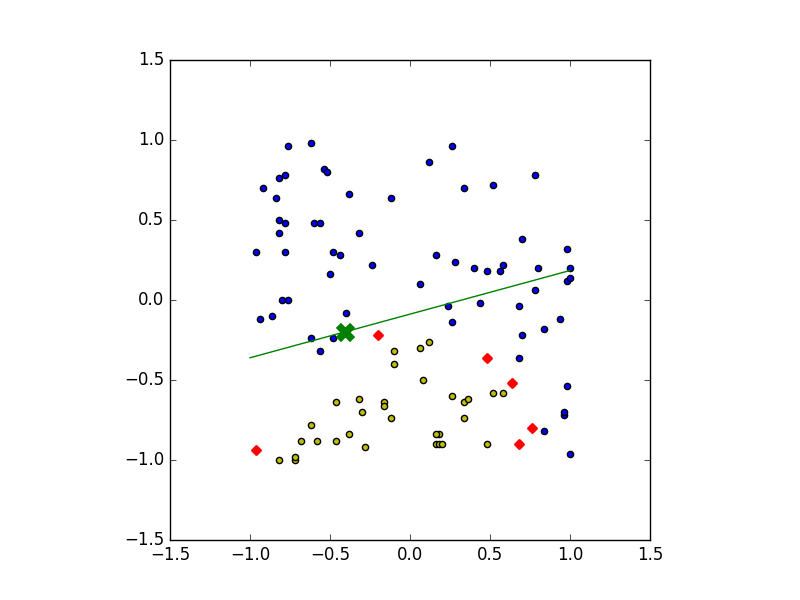
\includegraphics[width=\textwidth]{RBFN-BH-04.png}
    \caption{}
  \end{minipage}
  \hfill
\end{figure}

Unfortunately while its a lot closer than anything before still not quite the result we are looking for.

\section{Gated Neurons}
We now wish to move away from the idea of RFB Neurons and generalize our concept of a RBF Boundary Hunter Neuron to what we will call a \textbf{Gated Neuron}. This will allow us to define different methods for gating our neurons

\theoremstyle{definition}
\begin{definition}
A \textbf{Gated Neuron} has a \textbf{gating function} $g$ and prediction function $f$. $g$ takes the neurons input and outputs our certainty about the classification for that point, if $g$ is 0 then we are completely unsure about the input and if $g$ is 1 then we are certain. The Gated Neuron activation function is defined below

\begin{align}
a(x) &= \sigma(g(x) \cdot f(x))
\end{align}

\textbf{Note: } Equation (5.2) is not equivalent to our previous activation (5.1), we have moved the gating operation to inside the sigmoid function as this is simpler.

\end{definition}

\section{Hyperplane Gated Neuron}
We wish now to define a gated neuron which uses a hyperplane as to decide what it cares about, in a similar fashion to before we will define this gated neuron with a centre point.

\theoremstyle{definition}
\begin{definition}
A \textbf{Hyperplane Gated Neuron} is a gated neuron with the following parameters and functions. We have a point in our space $c$ (the centre of our gated neuron), and two hyperplanes which pass through this centre point, with normals $n$ and $m$. $n$ is the normal vector to the decision boundary and $m$ is the normal vector to a hyperplane which divides the plane into points we do and don't care about. Therefore giving us $g = \sigma(m \cdot (c - x))$ and $f = n \cdot (c - x)$. Now we can define the activation of such a neuron.

\begin{align}
a(x) = \sigma(\sigma(m \cdot (c - x)) \cdot (n \cdot (c - x)))
\end{align}

\end{definition}

Which then when trained on our chevron data gives the following result

\begin{figure}[H]
  \centering
  \begin{minipage}[b]{0.4\textwidth}
    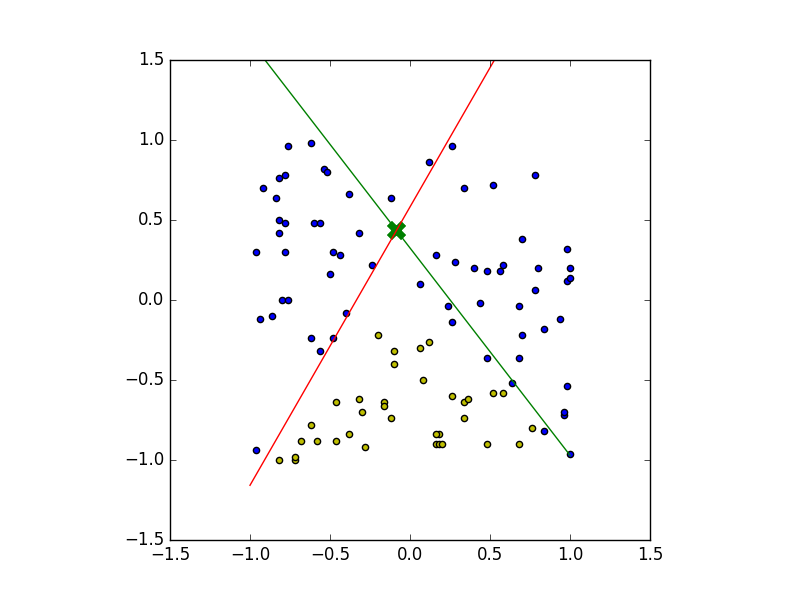
\includegraphics[width=\textwidth]{GN-MH-01.png}
    \caption{}
  \end{minipage}
  \hfill

The red line represents the gating hyperplane and the green line represents the decision boundary
\end{figure}

This is precisely what we are looking for in terms of classifying a chevron with only one boundary hunter.

\subsection{Comparison To Perceptron}
It should be noted that these boundary hunters require $3n$ parameters, a little less than three times the number required for a regular perceptron. The next reasonable question to ask is what can we achieve with a three layer perceptron network? We will compare our boundary hunter and three layer perceptron network's. The perceptron network will consist of three hidden neurons and 1 output neuron as these two network configurations have a similar amount of free parameters. We will compare their performance over the chevron dataset, using 10-Fold Cross Validation and computing a 95\% confidence interval on the accuracies to compare performance.

\begin{center}
\begin{tabular}{| c | c | c |}
\hline
Network & Avg Training Error & Avg Test Error \\
\hline
\hline
Perceptron & 0.00749882335194 & 0.0172678373009 \\
\hline
Gated Neuron & 0.0244635285134 & 0.0354204954447 \\
\hline
\end{tabular}
\end{center}

\begin{center}
\begin{tabular}{| c | c | c |}
\hline
Network & Training Error Conf Interval & Avg Test Error Conf Interval\\
\hline
\hline
Perceptron & (0.007, 0.008) & (0.007, 0.028)\\
\hline
Gated Neuron & (0.014, 0.035) & (0.012, 0.059)\\
\hline
\end{tabular}
\end{center}

These 95\% confidence intervals show that there is a statistically significant difference between the training but not the test accuracies, so we can conclude that the two methods have the same performance.

\subsection{Redundancy}
As part of the definition of our Hyperplane Gated Neuron we included a centre point, which is redundant. The point is essentially specifying the intersection of our two lines but this is not needed. We can remove this point and achieve the same results but with fewer free parameters, only 2n + 2 to be precise.

\begin{figure}[H]
  \centering
  \begin{minipage}[b]{0.8\textwidth}
    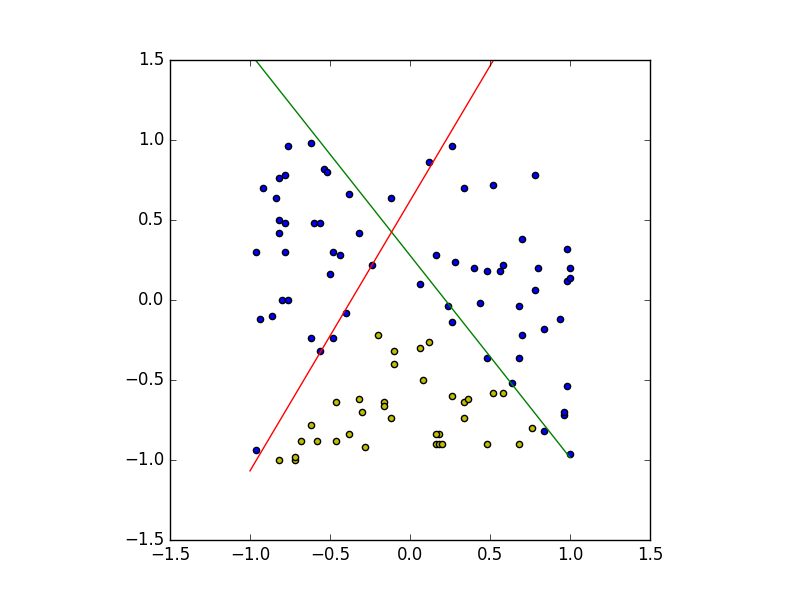
\includegraphics[width=\textwidth]{GN-MH-ONLY-01.png}
    \caption{}
  \end{minipage}
  \hfill

Hyperplane Gated Boundary Hunter without the centre point
\end{figure}

Comparing the performance of these new hyperplane gated boundary hunters against a standard perceptron network with 2 hidden neurons we get the following results

\begin{center}
\begin{tabular}{| c | c | c |}
\hline
Network & Avg Training Error & Avg Test Error \\
\hline
\hline
Perceptron & 0.023 & 0.037 \\
\hline
Gated Neuron & 0.023 & 0.031 \\
\hline
\end{tabular}
\end{center}

\begin{center}
\begin{tabular}{| c | c | c |}
\hline
Network & Training Error Conf Interval & Avg Test Error Conf Interval\\
\hline
\hline
Perceptron & (0.010, 0.037) & (0.013, 0.061)\\
\hline
Gated Neuron & (0.017, 0.030) & (0.008, 0.053)\\
\hline
\end{tabular}
\end{center}

With this modification we still find no statistically significant difference between the performance of our two networks, however the gated neuron network as the advantage that in low dimensions we can better understand how the network is breaking up the problem.

\subsection{Discussion}
We would like to ask ourselves, does our current solution solve the problem laid out in the beginning. How is this solution different to the one proposed in \cite{jacobs1991adaptive}. Our goal was to create neurons which act independently and learn to classify local features of the data.\\

Compared to the adaptive networks of experts it would definitely appear that we have created something with less dependency between the hidden neurons. In an adaptive network one neuron is only allowed slack off and get some things wrong if another neuron is picking up the slack and getting the points right. In our network each neuron is responsible for deciding what its interested in and it does not care what anything else is doing.\\

One thing to consider however is that out network has an output layer, taking the classification from each of the boundary hunters and making a final decision about what our network is going to say, this reintroduces some dependency between the hidden neurons. We can make this fact apparent by observing the following example, the data we are training over is rectangle boundary. In the case with one boundary hunter a reasonable attempt is made to classify the data, but the hunter struggles to place its self on a boundary,

\begin{figure}[H]
  \centering
  \begin{minipage}[b]{0.8\textwidth}
    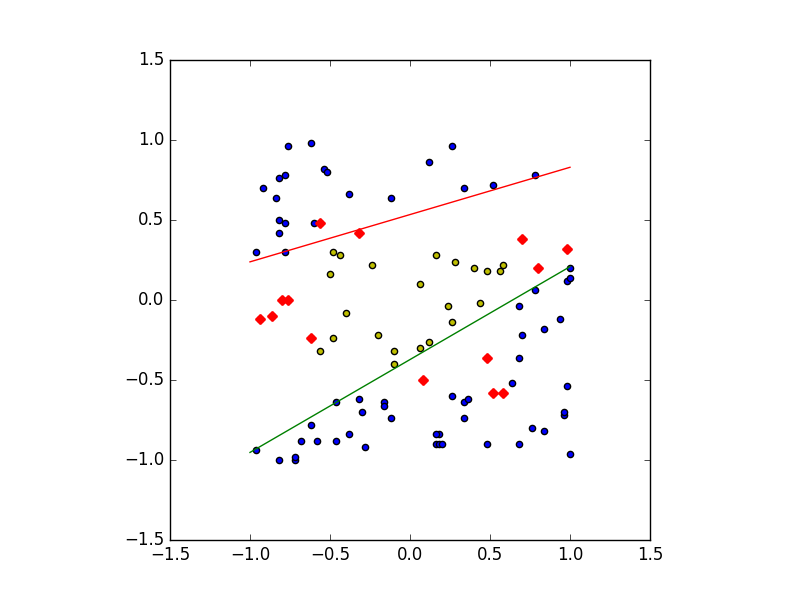
\includegraphics[width=\textwidth]{RecData-1HP.png}
    \caption{}
  \end{minipage}
  \hfill

Rectangle data trained with a single boundary hunter
\end{figure}

which when compared to the result training two boundary hunters on the same data definitely shows that there is some collaboration between the boundary hunters as none of them converge on the same solution as the single one did.

\begin{figure}[H]
  \centering
  \begin{minipage}[b]{0.8\textwidth}
    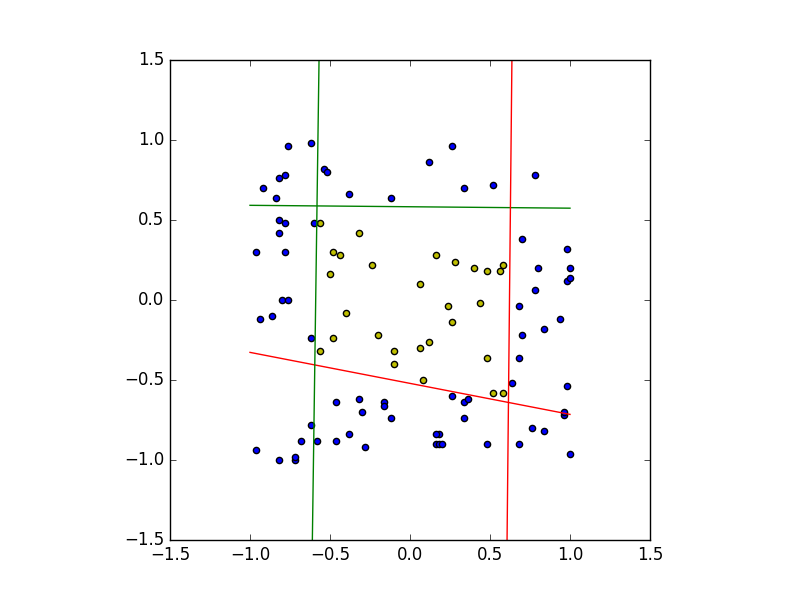
\includegraphics[width=\textwidth]{RecData-2HP.png}
    \caption{}
  \end{minipage}
  \hfill

Rectangle data trained with two boundary hunter
\end{figure}

A question that now seems logical to ask is, can we remove the output neuron and achieve the same results, thus further removing dependency between the neurons?

\chapter{Individual Hyperplane Gated Neurons}
In this chapter we work towards answering the question, can we train hyperplane gated neurons individually and achieve similar results the networks of such neurons. This has a very familiar feel to it, and is in fact close to our first attempt at creating a loss just a different way of computing responsibility. Because of this we are not surprised when we see that training this set-up has the same effect as what happened when using the loss function (3.3), our boundary hunter decided to care about everything.\\

Like before this result makes sense, if the boundary hunter can get away with getting everything right except say, 8 points, then this will have a lower error that getting penalised for not knowing half the points but getting everything it cares about right. Like before we see that not caring about a data point costs us $log(\frac{1}{2})$ which over a few points is a higher cost than simply a few wrong\\

\begin{figure}[H]
  \centering
  \begin{minipage}[b]{0.8\textwidth}
    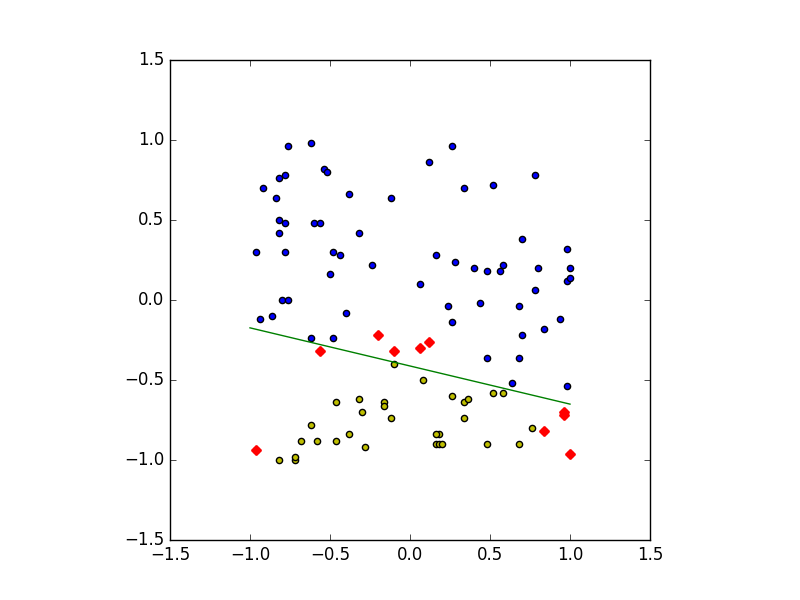
\includegraphics[width=\textwidth]{CHEVData-SingleBH.png}
    \caption{}
  \end{minipage}
  \hfill

Chevron data trained with a lone boundary hunter
\end{figure}

We now face the same issues as before, we need to provide a reward for ignoring data points, but how can we reward just enough without encouraging the boundary hunter to just ignore everything.

\section{Biases}
Currently our boundary hunter will take output a fair coin flip if it does not care about the data point. However this results in uninteresting solutions. It makes more sense for a boundary hunter to learn the value which they output in the case they don't care, we will call this parameter the bias $\beta$. Like before we have $g = \sigma(m \cdot (c - x))$ and $f = n \cdot (c - x)$. Now we can define the activation of such a neuron.

\begin{align}
a(x) = \sigma(g(x) \cdot f(x) + (1 - g(x)) \cdot \beta)
\end{align}

When training on the chevron data we now get almost the same output as when using the Gated Hyperplane Networks.

\begin{figure}[H]
  \centering
  \begin{minipage}[b]{0.8\textwidth}
    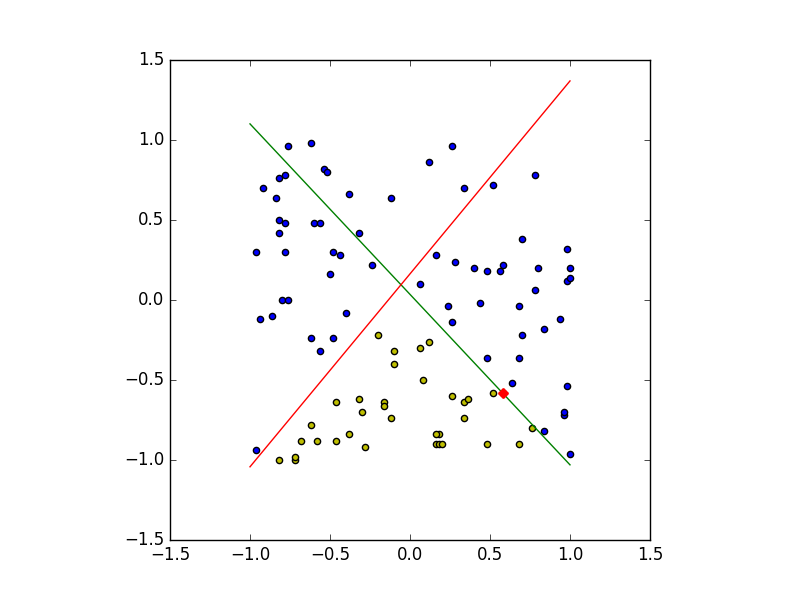
\includegraphics[width=\textwidth]{CHEVData-SingleBH-WithByas.png}
    \caption{}
  \end{minipage}
  \hfill

Chevron data trained with a lone boundary hunter with the learnable bias
\end{figure}

This is all very well but its very easy to learn the bias when there is only one class on the other side of our caring boundary, something more substantial would be if we could achieve these results but with a noisy dataset. Consider the following noisy chevron

\begin{figure}[H]
  \centering
  \begin{minipage}[b]{0.8\textwidth}
    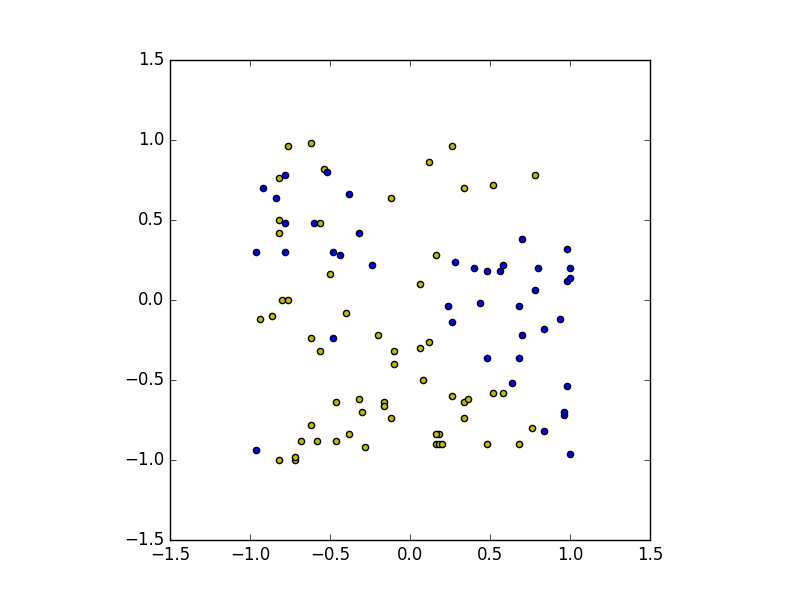
\includegraphics[width=\textwidth]{NoisyChev-RawData.png}
    \caption{}
  \end{minipage}
  \hfill
\end{figure}

With added noise the chevron becomes much less clear and could easily be interpreted in other ways, and while classifying the non noisy side of the chevron is still an option its not clear whether this is the best option. When trained the boundary hunter does not learn the side of the chevron but instead learns other boundary's in the data which with the added noise make a lot of sense.

\begin{figure}[H]
  \centering
  \begin{minipage}[b]{0.8\textwidth}
    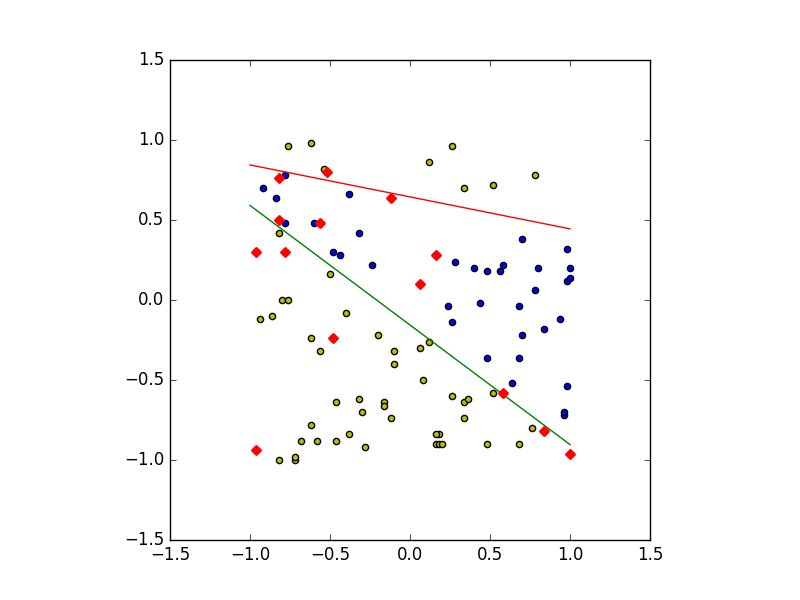
\includegraphics[width=\textwidth]{NoisyChev-BH-WithByas.png}
    \caption{}
  \end{minipage}
  \hfill
\end{figure}

Exactly what we wanted, getting a bunch of stuff wrong but on the other side of our caring boundary, everything we care about we are getting right. 

\chapter{Sonar Problem}
Given what we have achieved it would be interesting to see how this can perform on a real world data set with a lot more than 2 dimensions. The dataset we will consider is the \textbf{Sonar} dataset. This problem involves classification of sonar signals to determine whether they bounced off a rock or mine. This is a benchmark problem in machine learning so we have a good idea of what a good classification accuracy is. We will split the data set into training and test sets, given the total 208 data points, we randomly allocate 104 to the test set and the rest to training (the same split as \cite{gorman1988analysis} has). While it would of been nice to employ K-Fold Cross Validation due to time constraints this was not an option.\\

We will attempt to solve this problem using two different systems.

\begin{enumerate}
\item \textbf{Hoard of Boundary Hunters:} By training a number of individual boundary hunters on the data. Once all have been trained to classify a point we will employ a voting system, where a boundary hunter will give its best guess about the class of a point if it cares about the point otherwise it will abstain.

\item \textbf{Boundary Hunter Network:} By training a Hyperplane Gated Neuron Network on the data.
\end{enumerate}

While the main focus of this report was to develop the Hoard model it will be interesting to compare its performance to the Network model to determine what (if any) benefit having the output neuron provides.

\section{Results}
The performance of a Nearest Neighbour Classifier on this data is \textbf{82.7\%} and the best testing performance achieved so far is \textbf{90.4\%} on the test set \cite{gorman1988analysis}. When using a Boundary Hunter Network with 30 hidden neurons we where able to achieve \textbf{77\%} accuracy on the testing set, if we increase the number of boundary hunters to 50 we do not see any improvement, getting an accuracy of \textbf{79\%}.\\

When using our Hoard of Boundary Hunters system we where able to achieve \textbf{68\%} accuracy on the test set with 30 individually trained hunters, and an accuracy of \textbf{70\%} when using 50, so like before there is no significant change in performance. One benefit of these individual trained neurons is that they are able to tell us when they do not know something, when many have been combined together, like with what we have here, we end up in a situation where individually they do not take a guess at every data point but as a collective they do. What we would ideally see, in the case with 30 boundary hunters, is that the hoard collectively was unsure abut \textbf{31\%} of the test data but had a perfect accuracy on the parts of the test data which it was sure.\\

One possible benefit the output neuron provides is keeping the neurons away from each other, a reason for the better performance in the Network model. In the Hoard model our boundary hunters have no way to communicate and thus have no idea they are part of a collective, they simply think the only thing that matters is their accuracy and position themselves accordingly . The output neuron in the Network model provides a means for communication and perhaps encourages solutions where the boundary hunters are more spread out.

\chapter{Conclusion}
Locating local features in the data and ignoring everything else, a seemingly simple enough problem quickly became a difficult  balancing act of reward vs penalty. After multiple iterations of attempting to design a loss we concluded that this was not a promising avenue to follow.\\

Using the idea of RBF Networks we where able to develop similar models of boundary hunters but this was not quite solving the problem we had in mind, the network structure meant there was some dependency between our hidden neurons. Removing the network and individually training these boundary hunter neurons did not initially have the results we wanted, after adding biases which where learned along side the weights we started to see the kind of results we where looking for. Some tests on simple noisy data also proved promising.\\

Having our Boundary Hunters work on toy data is a good proof of concept but it is certainly not an accurate test of the performance for these neurons. Testing both individual and networks of boundary hunters on the Sonar benchmark problem showed that our ideas developed in this report do not give concepts which perform well enough to be effectively implemented in practice. Using either a Hoard or Network of boundary hunters does not provide better accuracy than a simple Nearest Neighbour Classifier. This suboptimal performance, is it caused simply because the base idea of a boundary hunter is flawed? or maybe our current attempt at one is unable to find all boundaries, meaning many neurons converge to the same position. We do not have enough information to make a determination on this point, however this is certainly an important question to be answered.\\

Our Hoard of Boundary Hunters model is a first attempt at solving the problem presented in this report and has provided promising results on generated data, with and without noise. As it stands the Hoard model does not perform well enough to compete with today's top of the line neural networks. 

\section{Future Work}
The following list presents some possible directions for anyone interested in taking this idea further.

\begin{enumerate}
\item Implement performance tests of the current models using K-Means to get truer estimate of performance.
\item Investigate if boundary hunters tend to converge on the same solution and if so develop a technique for keeping them out of each others way. Does this change improve performance of ether the Hoard or Network of boundary hunters.
\end{enumerate}

\newpage
\bibliographystyle{acm}
\bibliography{references}

\end{document}
